% introduction.tex
% Updated January 6, 2013

\chapter{An Introduction to Combinatorics}\label{ch:intro}

As we hope you will sense right from the beginning, we believe that
combinatorial mathematics is one of the most fascinating and
captivating subjects on the planet.  Combinatorics is \textit{very}
concrete and has a wide range of applications, but it also has an
intellectually appealing theoretical side. Our goal is to give you a
taste of both. In order to begin, we want to develop, through a series
of examples, a feeling for what types of problems combinatorics addresses.

\section{Introduction}\label{s:intro:intro}

There are three principal themes to our course:

\begin{description}
\item[Discrete Structures] Graphs, digraphs, networks, designs, posets, 
strings, patterns, distributions, coverings, and partitions.
\item[Enumeration] Permutations, combinations, inclusion/exclusion, 
generating functions, recurrence relations, and P\'olya counting. 
\item[Algorithms and Optimization] Sorting, spanning trees, shortest 
paths, eulerian circuits, hamiltonian cycles, graph coloring, 
planarity testing, network flows, bipartite matchings, and chain partitions. 
\end{description}

To illustrate the accessible, concrete nature of combinatorics and to
motivate topics that we will study, this preliminary chapter provides
a first look at combinatorial problems, choosing examples from
enumeration, graph theory, number theory, and optimization.  The
discussion is very informal---but this should serve to explain why we
have to be more precise at later stages.  We ask lots of questions,
but at this stage, you'll only be able to answer a few.  Later, you'll
be able to answer many more \dots but as promised earlier, most likely
you'll never be able to answer them all.  And if we're wrong in making
that statement, then you're certain to become \textit{very} famous.
Also, you'll get an A$++$ in the course and maybe even a Ph.D. too.

\section{Enumeration}\label{s:intro:enum}

Many basic problems in combinatorics involve counting the
number of distributions of objects into cells---where we may
or may not be able to distinguish between the objects and the
same for the cells.  Also, the cells may be arranged in patterns.
Here are concrete examples.

Amanda has three children: \quad Dawn, Keesha and Seth.

\begin{enumerate}
\item Amanda has ten one dollar bills and decides to give the full
  amount to her children.  How many ways can she do this?  For
  example, one way she might distribute the funds is to give Dawn and
  Keesha four dollars each with Seth receiving the balance---two
  dollars.  Another way is to give the entire amount to Keesha, an
  option that probably won't make Dawn and Seth very happy.  Note that
  hidden within this question is the assumption that Amanda does not
  distinguish the individual dollar bills, say by carefully examining
  their serial numbers.  Instead, we intend that she need only
  decide the \textit{amount} each of the three children is to receive.
  
\item  The amounts of money distributed to the three children form a
sequence which if written in non-increasing order has the form:\quad
$a_1, a_2, a_3$ with $a_1\ge a_2\ge a_3$ and $a_1+a_2+a_3=10$.  How many
such sequences are there?
\item Suppose Amanda decides to give each child at least one dollar.  How
does this change the answers to the first two questions?
\item Now suppose that Amanda has ten books, in fact the top 10 books from the New
York Times best-seller list, and decides to give them to her
children.  How many ways can she do this?  Again, we note that there is
a hidden assumption---the ten books are all different.
\item Suppose the ten books are labeled $B_1, B_2,\dots, B_{10}$.
The sets of books given to the three children are pairwise disjoint and
their union is $\{B_1,B_2,\dots,B_{10}\}$.  How many different sets of 
the form $\{S_1, S_2, S_3\}$ where $S_1$, $S_2$ and $S_3$ are pairwise
disjoint and $S_1\cup S_2\cup S_3=\{B_1,B_2,\dots,B_{10}\}$?
\item Suppose Amanda decides to give each child at least one book.  How
does this change the answers to the preceding two questions?
\item How would we possibly answer these kinds of questions if ten 
was really ten thousand (OK, we're not talking about children any more!)
and three was three thousand?  Could you write the answer on a single
page in a book?
\end{enumerate}

A circular necklace with a total of six beads will be assembled using beads
of three different colors.  In \autoref{fig:intro:necklace}, we show four such
necklaces---however, note that the first three are actually the \textit{same}
necklace.  Each has three red beads, two blues and one green.  On the 
other hand, the fourth necklace has the same number of beads of each color but
it is a \textit{different} necklace.

\begin{figure}
\begin{center}
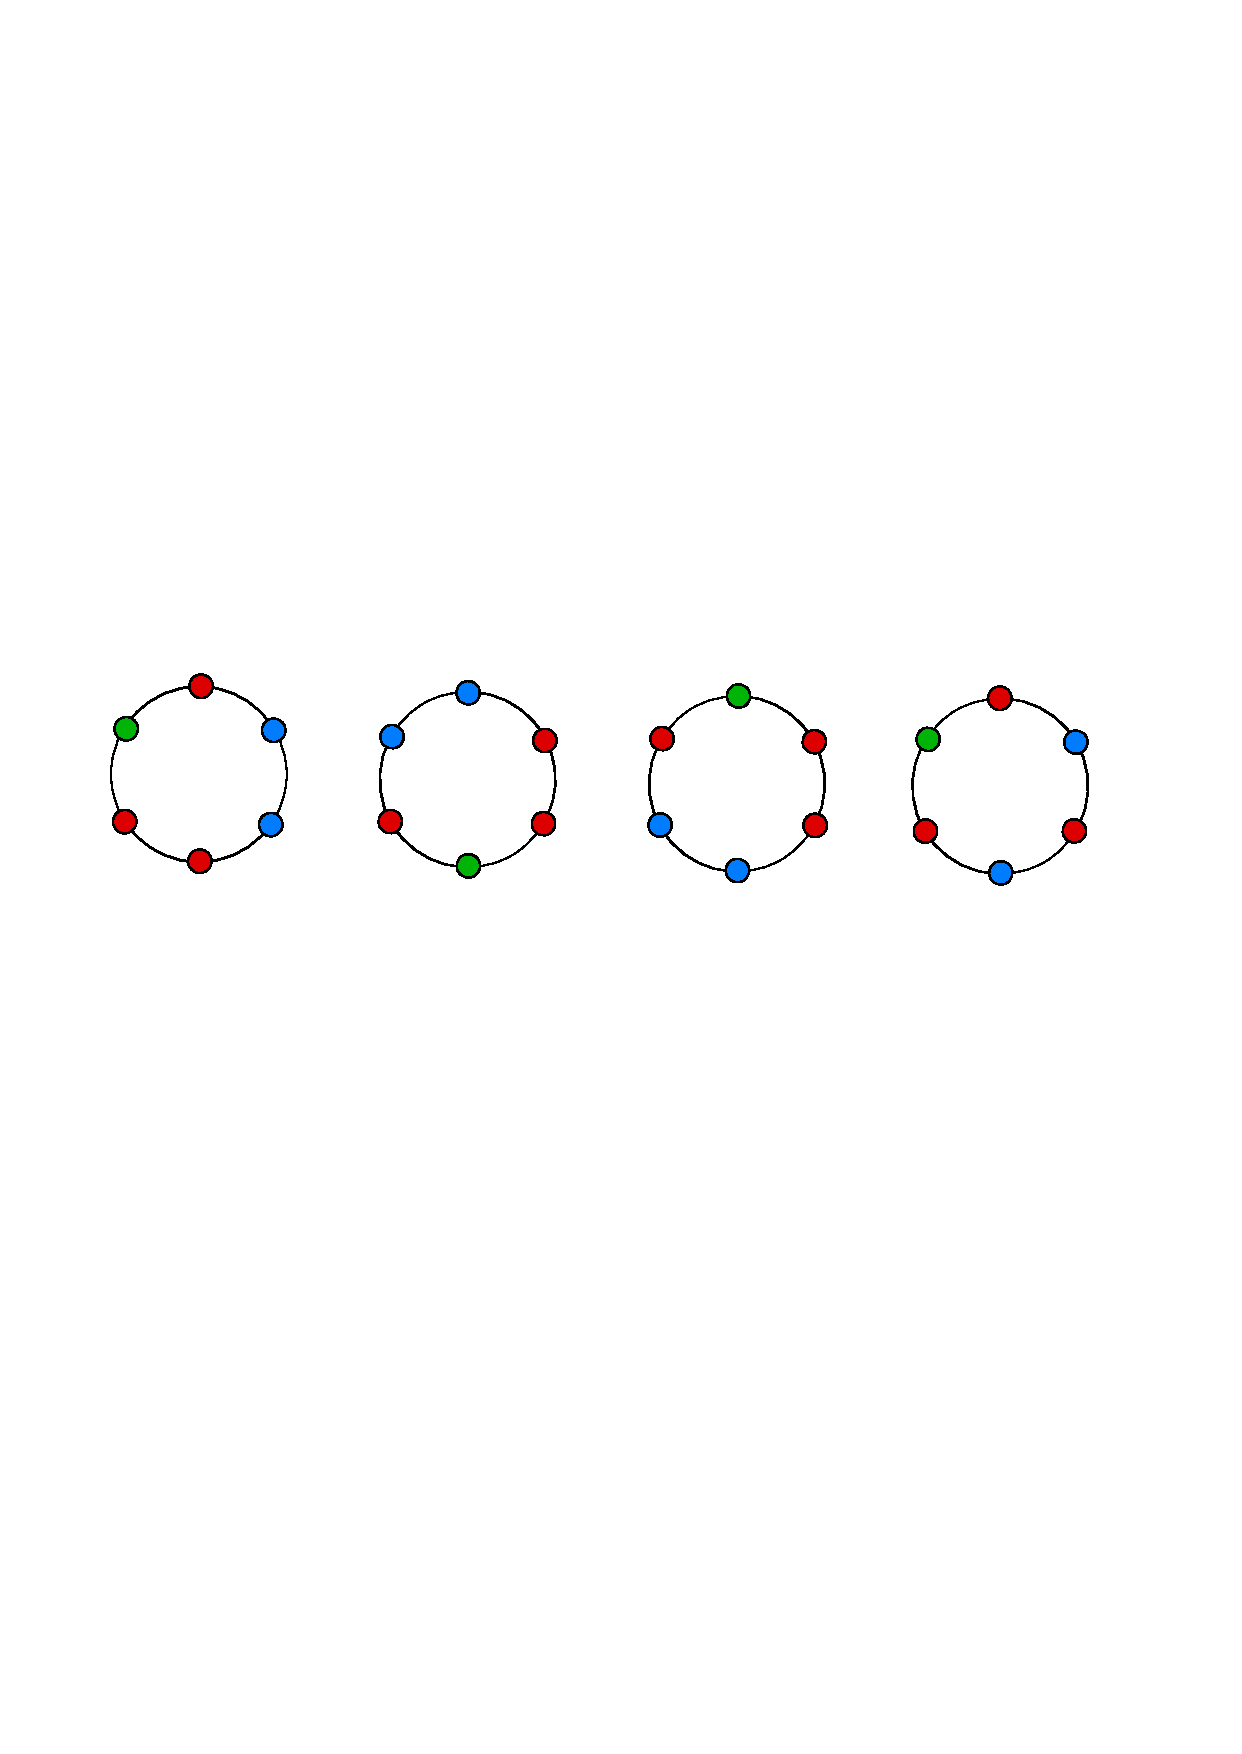
\includegraphics[viewport=44 401 537 528, scale=.6]{intro-figs/necklaces}\\
\caption{Necklaces made with three colors} 
\label{fig:intro:necklace}
\end{center}
\end{figure}


\begin{enumerate}
\item How many different necklaces of six beads can be formed using three reds, two
blues and one green?
\item How many different necklaces of six beads can be formed using red, blue and green
beads (not all colors have to be used)?
\item How many different necklaces of six beads can be formed using red, blue and green
beads if all three colors have to be used?
\item How would we possibly answer these questions for necklaces of six 
thousand beads made with beads from three thousand different colors?
What special software would be required to find the exact answer and how
long would the computation take?
\end{enumerate}

\section{Combinatorics and Graph Theory}\label{s:intro:graph}

A \textit{graph} $G$ consists of a \textit{vertex} set $V$ and
a collection $E$ of $2$-element subsets of $ V$. Elements of $E$ are
called edges.  In our course, we will (almost always) use the convention
that $V=\{1,2,3,\dots,n\}$ for some positive integer~$n$.  With
this convention, graphs can be described \textit{precisely}
with a text file:
\begin{enumerate}
\item The first line of the file contains a single integer $n$, the
number of vertices in the graph.
\item Each of the remaining lines of the file contains a pair of 
distinct integers and specifies an edge of the graph.
\end{enumerate}
We illustrate this convention in \autoref{fig:graphdata} with a text 
file and the diagram for the graph~$G$ it defines.

\hspace{.5in}
\begin{figure}
\begin{minipage}{1.5in}
\texttt{graph1.txt}\\
9\\
6 2\\
1 5\\
1 7\\
6 8\\
9 1\\
4 3\\
5 7\\
1 3\\
5 9\\
7 9
\end{minipage}
\begin{minipage}{3in}
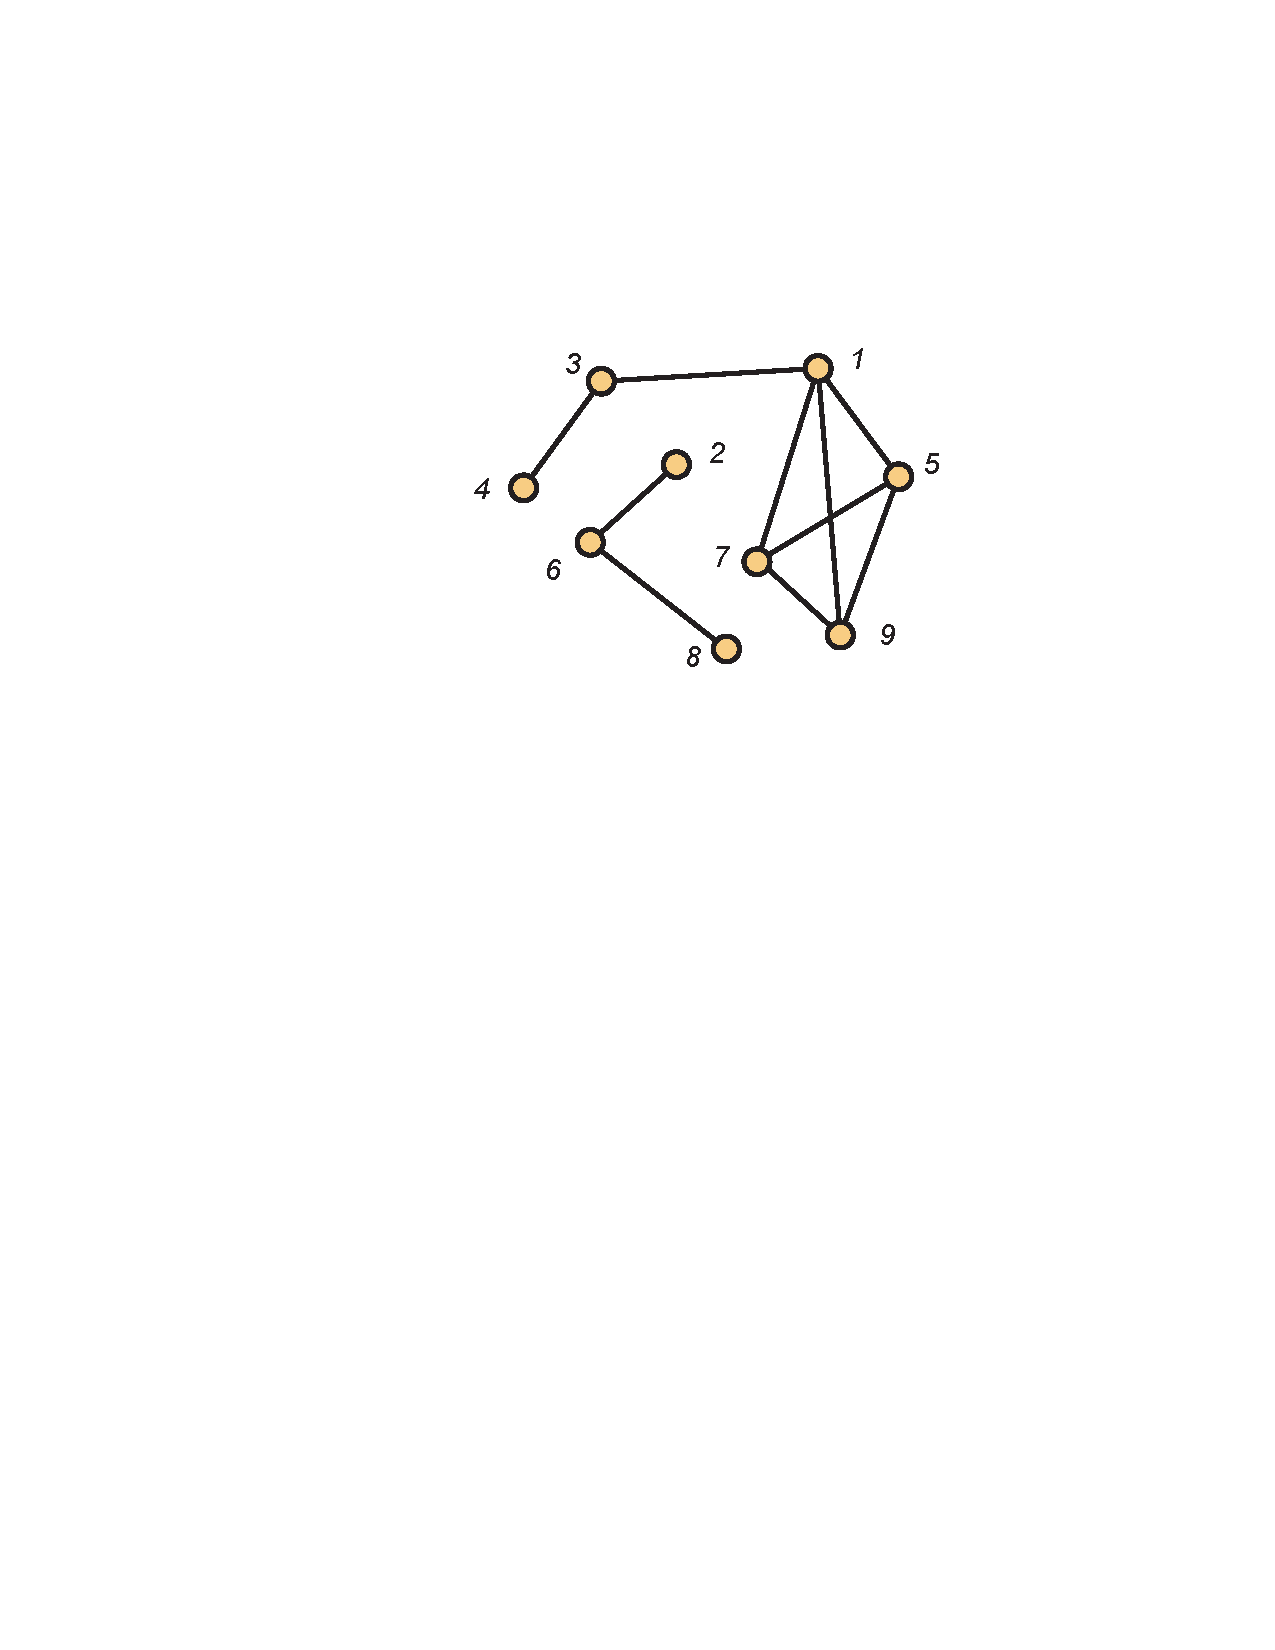
\includegraphics[viewport=223 457 460 629, scale=.6]{intro-figs/3012-fig15}\\
\caption{A graph defined by data}
\label{fig:graphdata}
\end{minipage}
\end{figure}

\medskip
Much of the notation and terminology for graphs is quite natural.
See if you can make sense out of the following statements which
apply to the graph $G$ defined above:
\begin{enumerate}
\item $G$ has $9$ vertices and $10$ edges.
\item $\{2,6\}$ is an edge.
\item Vertices $5$ and $9$ are adjacent.
\item $\{5,4\}$ is not an edge.
\item Vertices $3$ and $7$ are not adjacent.
\item $P = (4, 3,1, 7,9,5)$ is a path 
of length~$5$ from vertex $4$ to vertex~$5$.
\item $C=(5,9,7,1)$ is cycle of length~$4$.
\item $G$ is disconnected and has two components.
One of the components has vertex set $\{2,6,8\}$.
\item $\{1,5,7\}$ is a triangle.
\item $\{1,7,5,9\}$ is a clique of size~$4$.
\item $\{4,2,8,5\}$ is an independent set of
size~$4$.
\end{enumerate}

Equipped only with this little bit of background
material, we are already able to pose a number
of interesting and challenging problems.  

\begin{example}
Consider the graph $G$ shown in \autoref{fig:connectedgraph}.

\begin{figure}
\begin{center}
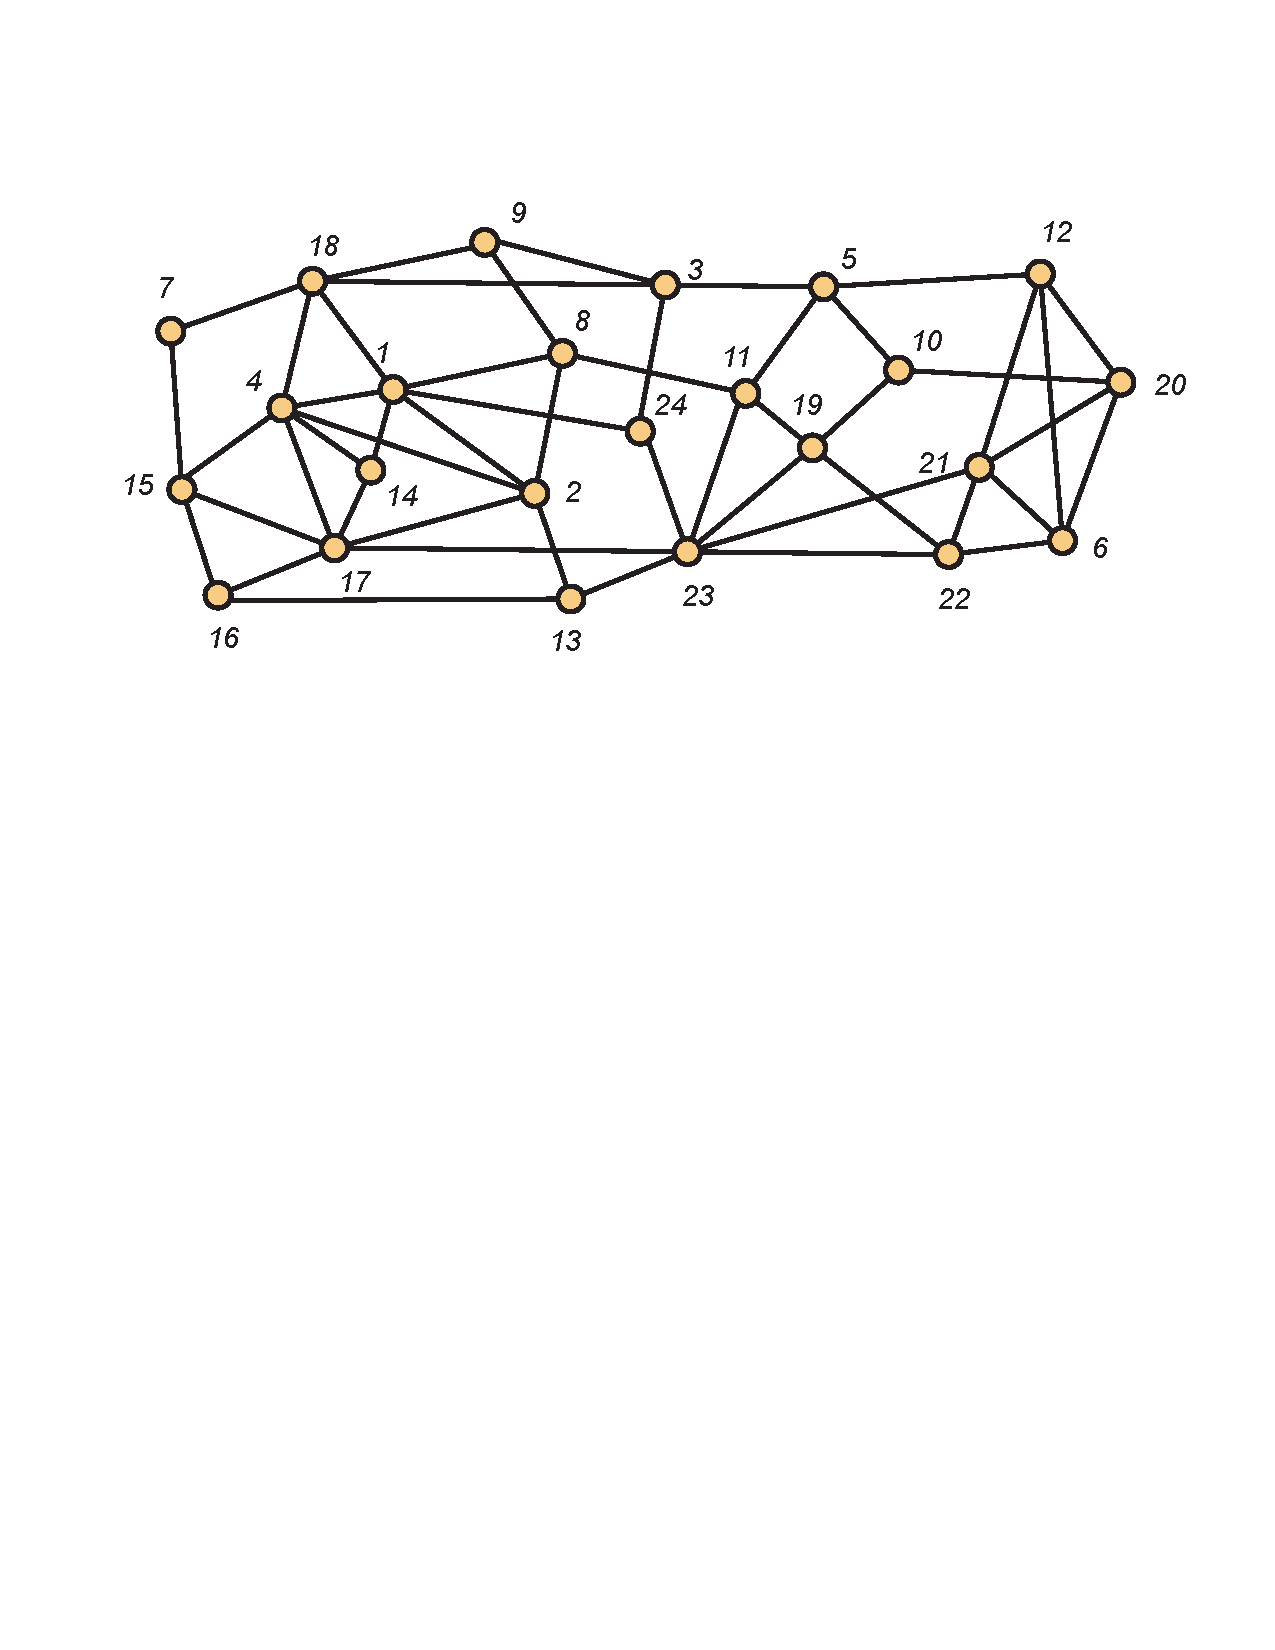
\includegraphics[viewport=55 462 575 702, scale=.6]{intro-figs/3012-fig17}\\
\caption{A connected graph}
\label{fig:connectedgraph}
\end{center}
\end{figure}

\begin{enumerate}
\item What is the largest $k$ for which $G$ has a path
of length~$k$? 
\item What is the largest $k$ for which $G$ has a cycle 
of length~$k$? 
\item What is the largest $k$ for which $G$ has a clique
of size~$k$? 
\item What is the largest $k$ for which $G$ has an
independent set of size~$k$? 
\item  What is the shortest path from vertex~$7$ to
vertex~$6$?
\end{enumerate}

Suppose we gave the class a text data file for a graph
on $1500$ vertices and asked whether the graph contains
a cycle of length at least $500$.  Raoul says yes and
Carla says no. How do we decide who is right?

Suppose instead we asked whether the graph has a clique of
size~$500$.  Helene says that she doesn't think so, but isn't
certain.  Is it reasonable that her classmates insist that
she make up her mind, one way or the other?  Is determining whether
this graph has a clique of size~$500$ harder, easier or
more or less the same as determining whether
it has a cycle of size~$500$.
\end{example}

We will frequently study problems in which graphs
arise in a very natural manner.  Here's an example.

\begin{example}\label{ex:radiostations}
In \autoref{fig:radiostations}, we show the location of some radio stations in the
plane, together with a scale indicating a distance of~$200$ miles.
Radio stations that are closer than~$200$ miles apart must broadcast
on different frequencies to avoid interference.  

\begin{figure}
\begin{center}
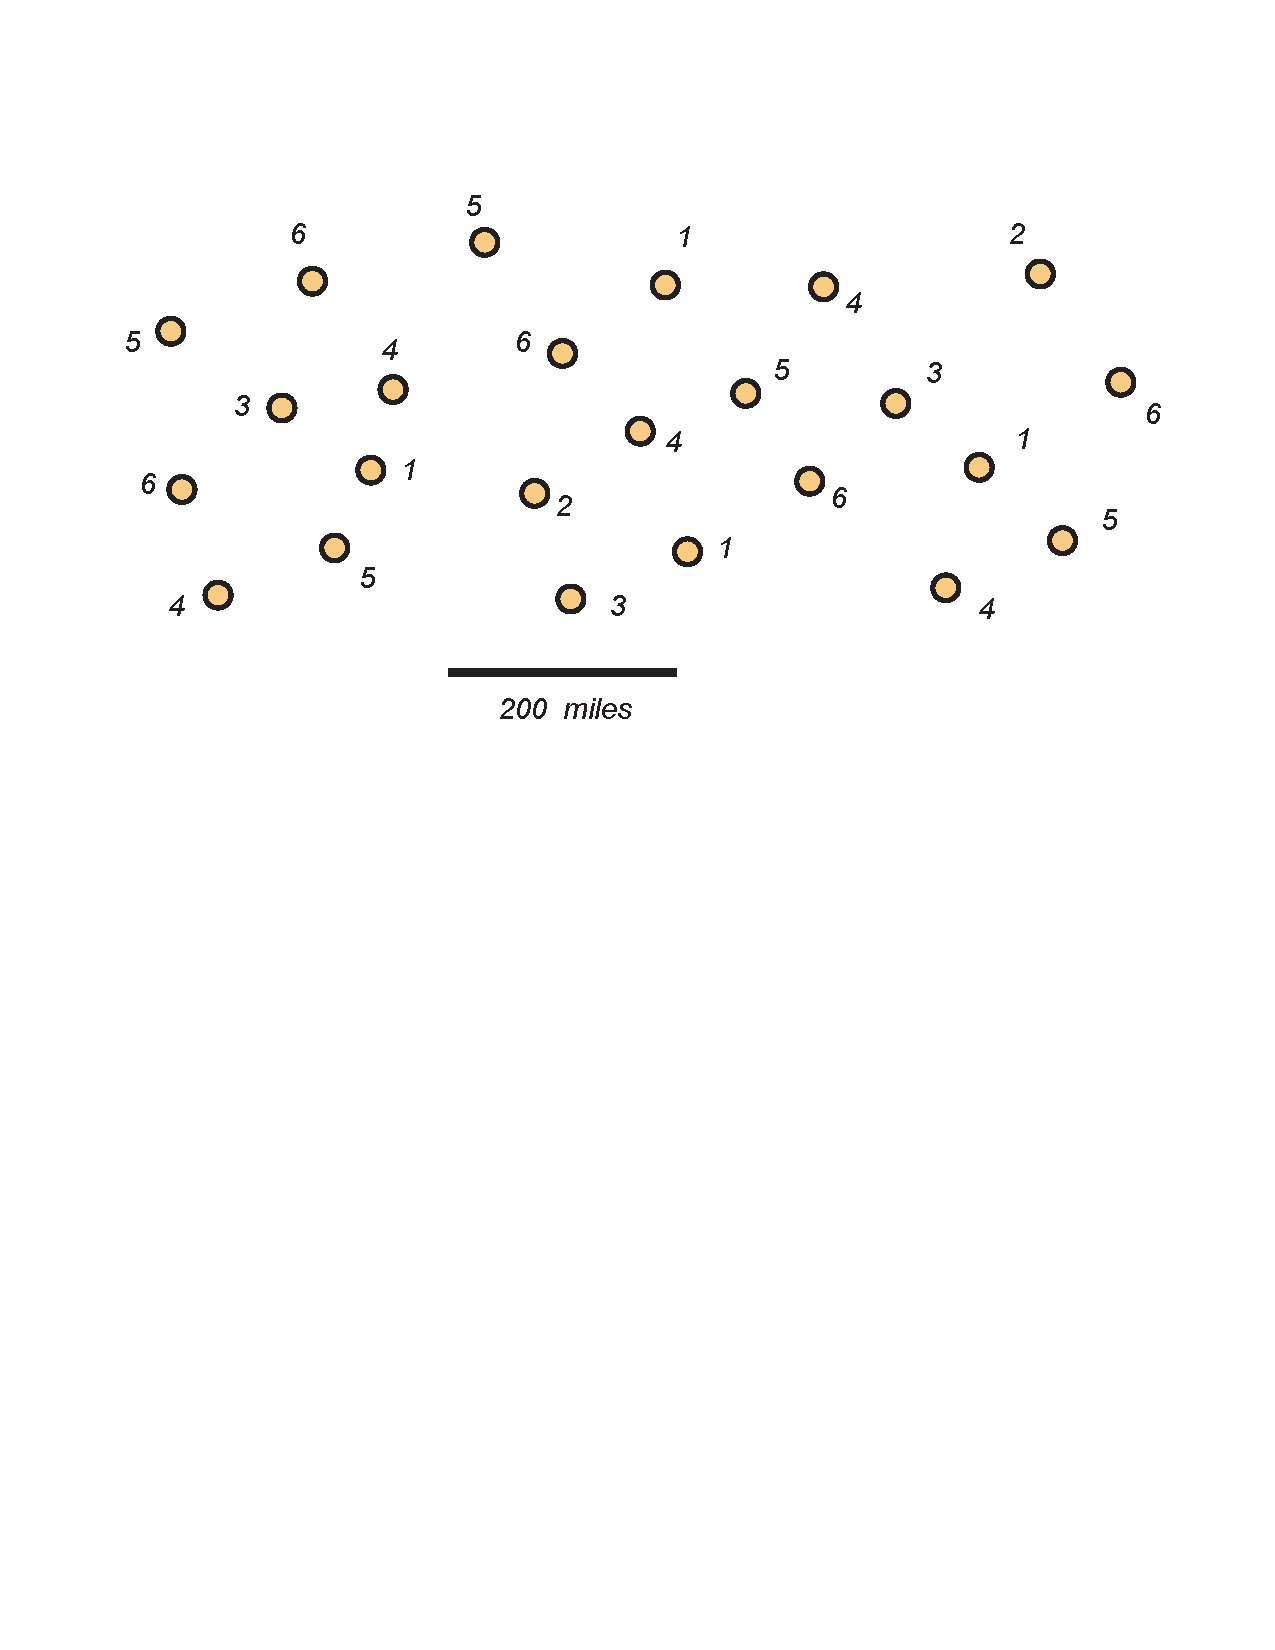
\includegraphics[viewport=46 433 576 706, scale=.6]{intro-figs/3012-fig4}\\
\end{center}
\caption{Radio Stations}
\label{fig:radiostations}
\end{figure}

We've shown that~$6$ different frequencies are enough.  
Can you do better?

Can you find~$4$ stations each of which is within
$200$ miles of the other~$3$?  Can you find $8$ stations each of is more
than $200$ miles away from the other~$7$?   Is there a natural
way to define a graph associated with this problem?
\end{example}

\begin{example}
How big must an applied combinatorics class be so that there are
either (a)~six students with each pair having taken at least one
other class together, or (b)~six students with each pair together
in a class for the first time.  Is this really a hard problem or
can we figure it out in just a few minutes, scribbling on a napkin?
\end{example}
 
\section{Combinatorics and Number Theory}\label{s:intro:number}

Broadly, number theory concerns itself with the properties of the
positive integers. G.H.\ Hardy was a brilliant British mathematician
who lived through both World Wars and conducted a large deal of
number-theoretic research. He was also a pacifist who was happy that,
from his perspective, his research was not ``useful''. He wrote in his
1940 essay \emph{A Mathematician's Apology} ``[n]o one has yet
discovered any warlike purpose to be served by the theory of numbers
or relativity, and it seems very unlikely that anyone will do so for
many years.''\footnote{G.H.\ Hardy, \textit{A Mathematician's
    Apology}, Cambridge University Press, p. 140. (1993 printing)}
Little did he know, the purest mathematical ideas of number theory
would soon become indispensable for the cryptographic techniques that
kept communications secure. Our subject here is not number theory, but
we will see a few times where combinatorial techniques are of use in
number theory.

\begin{example}\label{ex:collatz}
Form a sequence of positive integers using the
following rules.  Start with a positive integer $n>1$. If $n$ is odd,
then the next number is $3n+1$.  If $n$ is even, then the
next number is $n/2$.  Halt if you ever reach~$1$.
For example, if we start with $28$, the sequence is
\[
28, 14, 7, 22, 11, 34, 17, 52, 26, 13, 40, 20, 10, 5, 16, 8, 4, 2, 1.
\]

Now suppose you start with $19$.  Then the first few terms are
\[
19, 58, 29, 88, 44, 22.
\]
But now we note that the integer $22$ appears in the first sequence,
so the two sequences will agree from this point on.  Sequences formed
by this rule are called \textit{Collatz sequences}.

Pick a number somewhere between $100$ and $200$ and write down the sequence
you get.  Regardless of your choice, you will eventually halt with a~$1$.
However, is there some positive integer $n$ (possibly quite large) so
that if you start from $n$, you will never reach~$1$?
\end{example}
 
\begin{example}
Students in middle school are taught to add fractions by finding
least common multiples.  For example, the least common multiple
of $15$ and $12$ is $60$, so:

\[
\frac{2}{15}+ \frac{7}{12} = \frac{8}{60}+\frac{35}{60} = \frac{43}{60}.
\]

How hard is it to find the least common multiple of two integers?
It's really easy if you can factor them into primes.  For example,
consider the problem of finding the least common multiple
of $351785000$ and  $316752027900$ if you just happen to know that

\begin{align*}
 351785000 = & 2^3\times 5^4\times 7\times19\times 23^2\quad\text{and}\\ 
 316752027900 = & 2^2\times3\times 5^2\times 7^3\times 11\times 23^4. 
\end{align*}
Then the least common multiple is
\begin{align*}
300914426505000 = & 2^3\times3\times 5^4\times 7^3\times 11\times 19\times 23^4.
\end{align*}
So to find the least common multiple of two numbers, we just have
to factor them into primes.  That doesn't sound too hard. For starters, can you
factor $1961$?  OK, how about $1348433$?  Now for a real challenge.
Suppose you are told that the integer
\[
c = 5220070641387698449504000148751379227274095462521
\]
is the product of two primes $a$ and $b$.  Can you find them?

What if factoring is hard?  Can you find the least common multiple of
two relatively large integers, say each with about~$500$ digits, by
another method? How should middle school students be taught to add
fractions?

As an aside, we note that most calculators can't add or multiply two
$20$ digits numbers, much less two numbers with more than~$500$
digits.  But it is relatively straightforward to write a computer
program that will do the job for us.  Also, there are some powerful
mathematical software tools available.  Two very well known examples
are \emph{Maple}\textsuperscript{\tiny\textregistered} and
\emph{Mathematica}\textsuperscript{\tiny\textregistered}.  For example, if you open up a
\emph{Maple} workspace and enter the command:

\begin{center}
\texttt{ifactor(300914426505000)};
\end{center}
then about as fast as you hit the carriage return, you
will get the prime factorization shown above.

Now here's how we made up the challenge problem.  First, we found a
site on the web that lists large primes and found these two values:

\begin{align*}
a = & 45095080578985454453\quad\text{and}\\ 
b = & 115756986668303657898962467957.
\end{align*}
We then used \emph{Maple} to multiply them together using the following command:

\[
45095080578985454453*115756986668303657898962467957;
\]
Almost instantly, \emph{Maple} reported the value for $c$ given above.

Out of curiosity, we then asked \emph{Maple} to factor~$c$.  It took almost
$12$ minutes on a powerful desktop computer.
\end{example}

Questions arising in number theory can also have an enumerative flair,
as the following example shows.

\begin{example}
In \autoref{tab:intro:partsof8}, we show the integer partitions
of~$8$.
\begin{table}[hb]
\centering
\begin{tabular}{lll}
  8\quad\text{distinct parts}&
  7+1\quad\text{distinct parts, odd parts}&
  6+2\quad\text{distinct parts}\\
  6+1+1&
  5+3\quad\text{distinct parts, odd parts}&
  5+2+1\quad\text{distinct parts}\\
  5+1+1+1\quad\text{odd parts}&
  4+4&
  4+3+1\quad\text{distinct parts}\\
  4+2+2&
  4+2+1+1&
  4+1+1+1+1\\
  3+3+2&
  3+3+1+1\quad\text{odd parts}&
  3+2+2+1\\
  3+2+1+1+1&
  3+1+1+1+1+1\quad\text{odd parts}&
  2+2+2+2\\
  2+2+2+1+1&
  2+2+1+1+1+1&
  2+1+1+1+1+1+1\\&
  1+1+1+1+1+1+1+1\quad\text{odd parts}
\end{tabular}
\caption{The partitions of $8$, noting those into distinct parts
  and those into odd parts.}
\label{tab:intro:partsof8}
\end{table}
There are~$22$ partitions altogether, and as noted, exactly~$6$
of them are partitions of~$8$ into odd parts.  Also, exactly~$6$ of them
are partitions of~$8$ into distinct parts.

What would be your reaction if we asked you to find the number of
integer partitions of $25892$?  Do you think that the number of
partitions of $25892$ into odd parts equals the number of partitions
of $25892$ into distinct parts?  Is there a way to answer this
question \textit{without} actually calculating the number of
partitions of each type?
\end{example}

\section{Combinatorics and Geometry}\label{s:intro:geom}

There are many problems in geometry that are innately combinatorial or
for which combinatorial techniques shed light on the problem.

\begin{example}  
  In \autoref{fig:linesregions}, we show a family of $4$ lines in
  the plane.  Each pair of lines intersects and no point in the plane
  belongs to more than two lines.  These lines determine~$11$ regions.

\begin{figure}[hbt]
\begin{center}
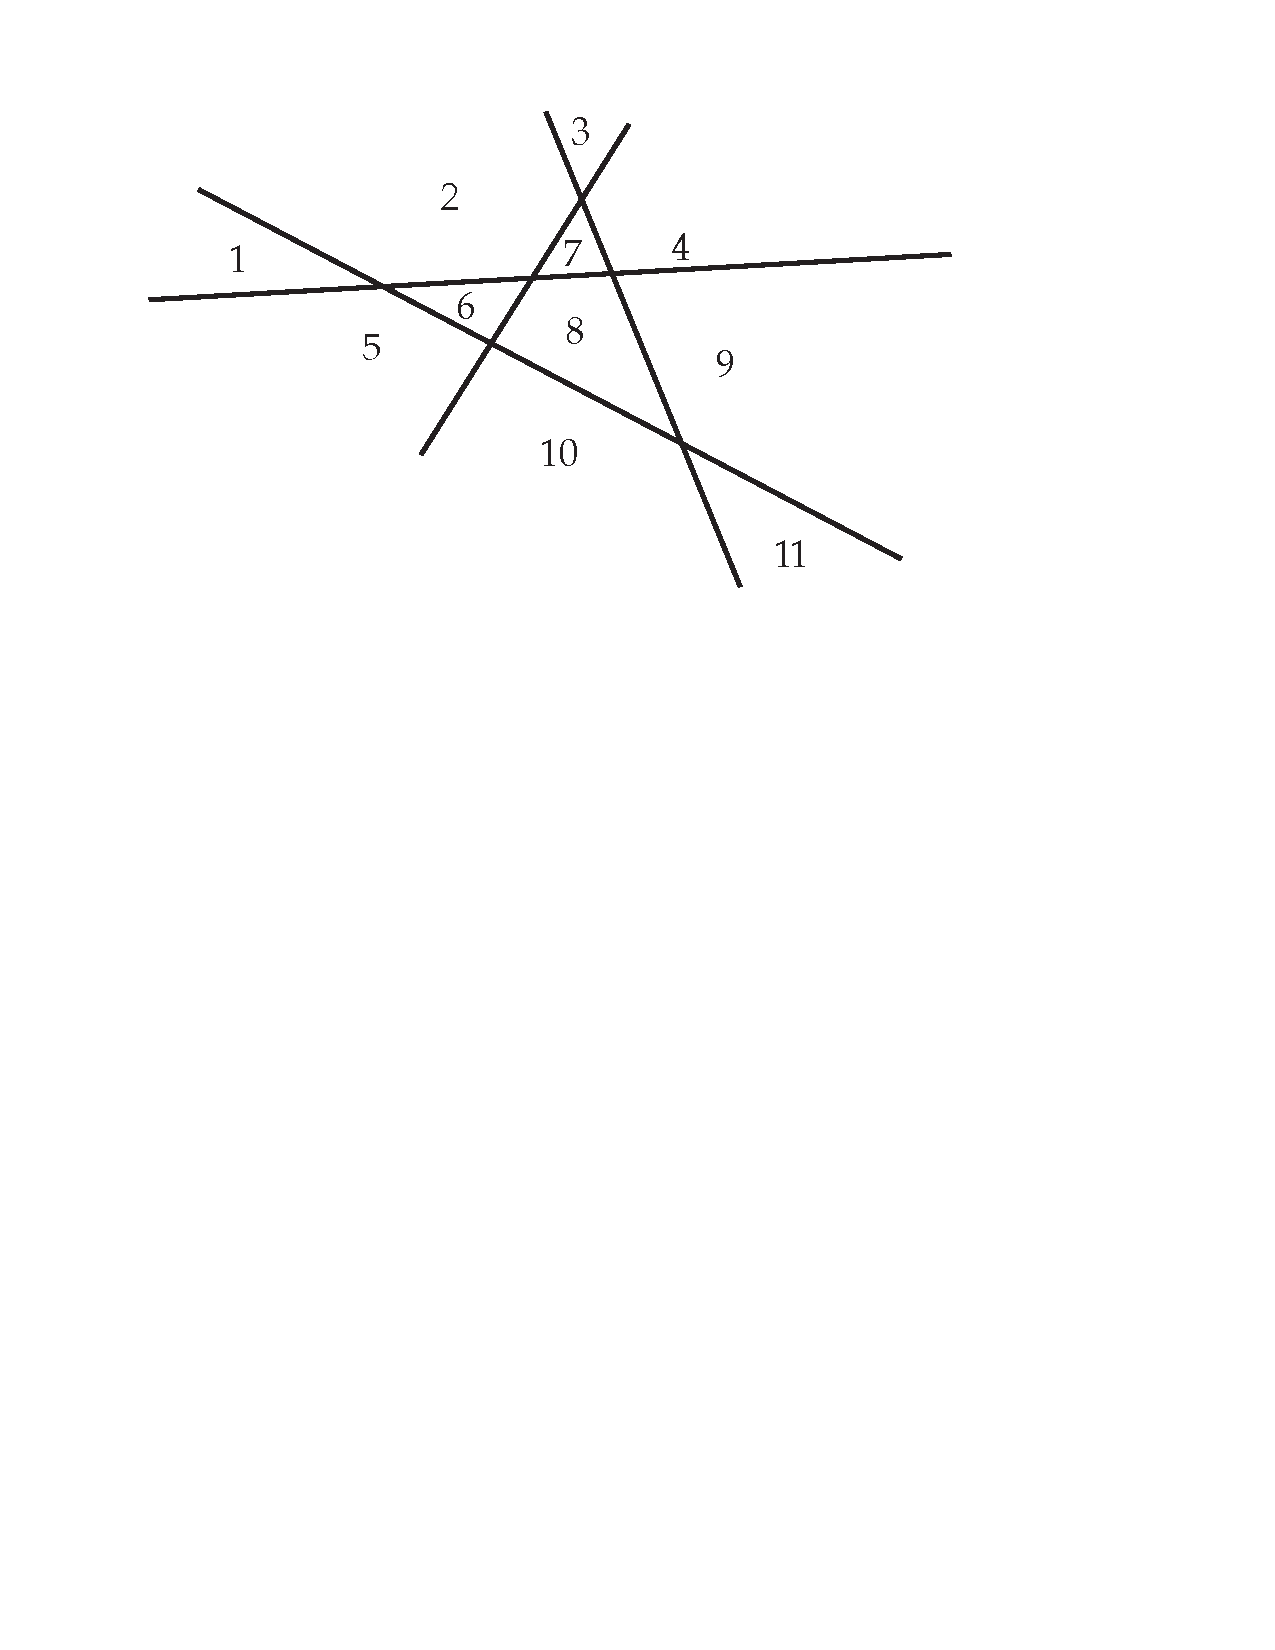
\includegraphics[viewport=60 480 470 745, scale=.6]{intro-figs/3012-fig9}\\
\end{center}
\caption{Lines and regions}
\label{fig:linesregions}
\end{figure}

Under these same restrictions, how many regions would a family of
$8947$ lines determine?  Can different arrangements of lines determine
different numbers of regions?
\end{example}

\begin{example}
Mandy says she has found a set of~$882$ points in the plane that
determine exactly $752$ lines.  Tobias disputes her claim.
Who is right?
\end{example}

\begin{example}
There are many different ways to draw a graph in the plane. Some
drawings may have crossing edges while others don't.  But sometimes, crossing
edges must appear in any drawing.
Consider the graph $G$ shown in \autoref{fig:crossingedges}.
\begin{figure}
\begin{center}
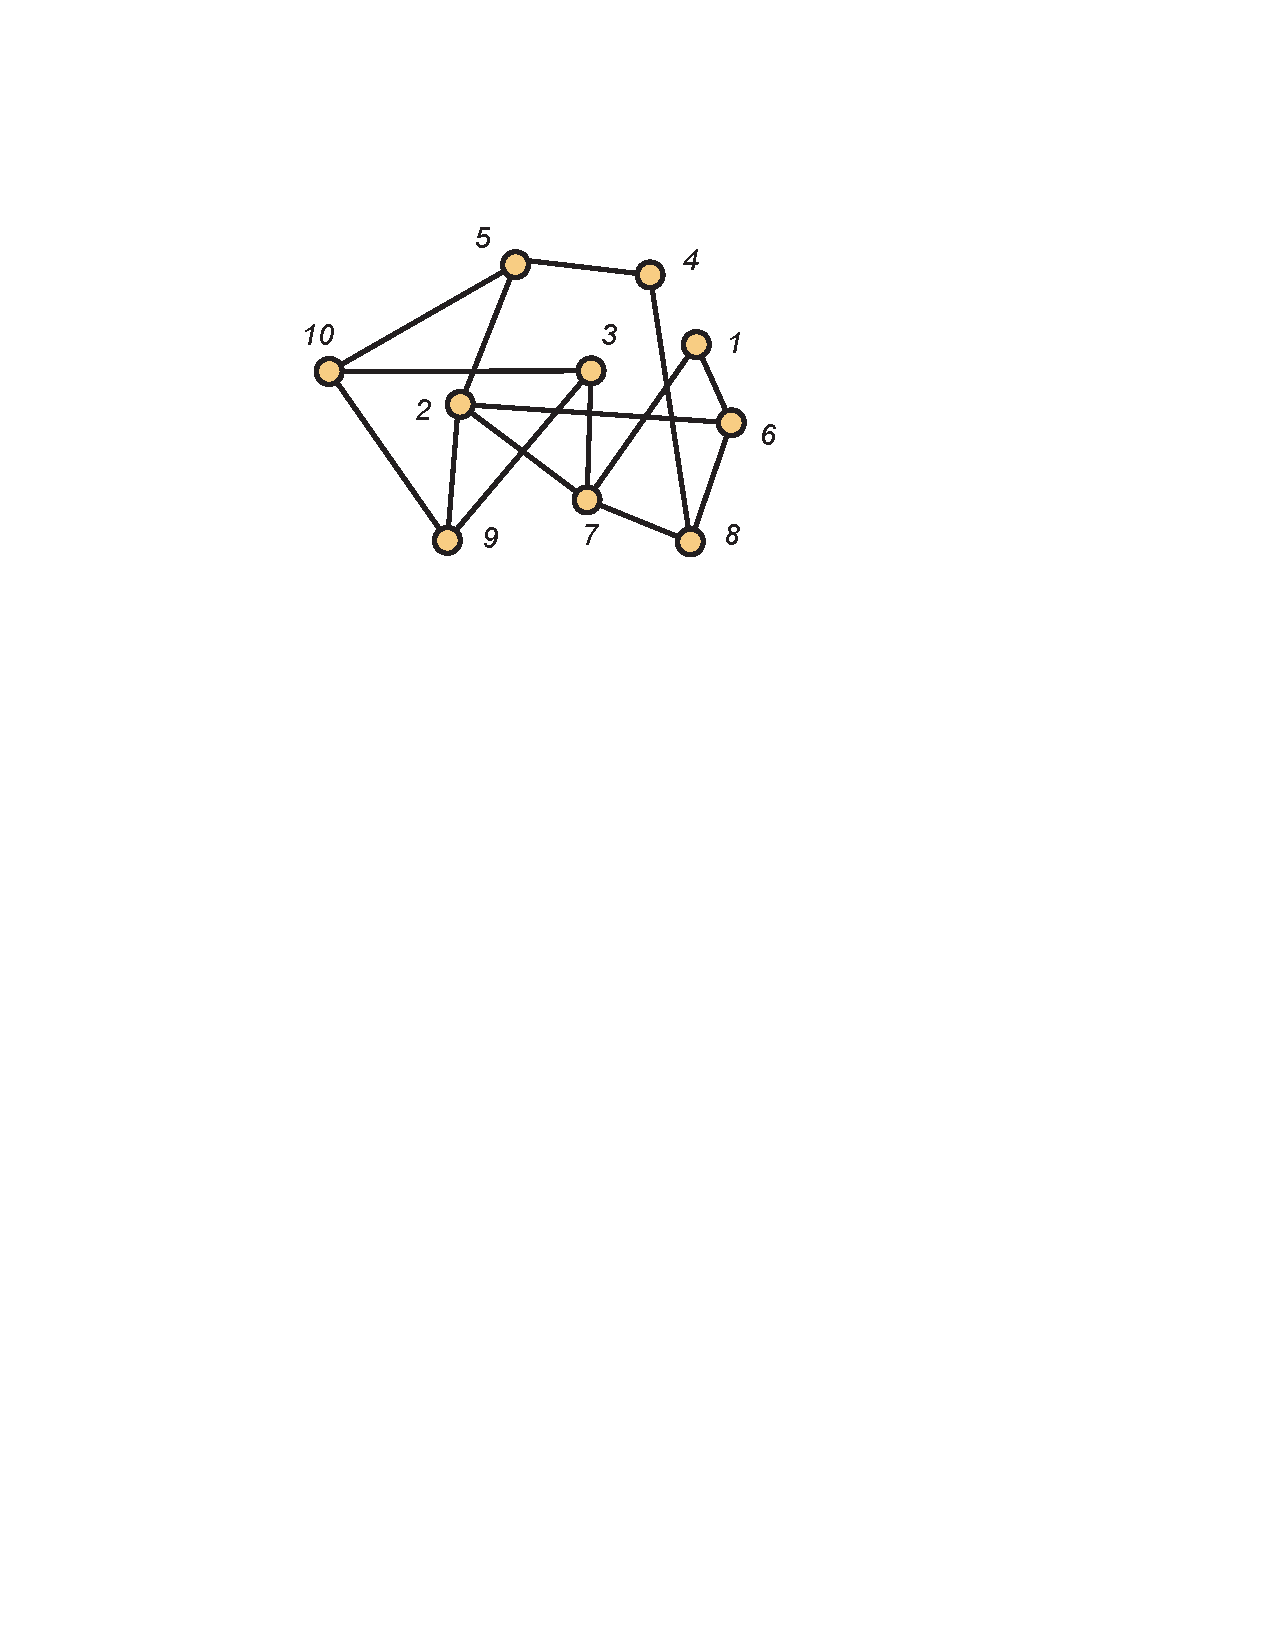
\includegraphics[viewport=132 509 372 683, scale=.6]{intro-figs/3012-fig8}\\
\end{center}
\caption{A graph with crossing edges}
\label{fig:crossingedges}
\end{figure}
Can you redraw $G$ without crossing edges?

Suppose Sam and Deborah were given a homework problem asking whether a
particular graph on $2843952$ vertices and $9748032$ edges could be
drawn without edge crossings.  Deborah just looked at the number of
vertices and the number of edges and said that the answer is ``no.''
Sam questions how she can be so certain---without looking more
closely at the structure of the graph.  Is there a way for
Deborah to justify her definitive response?
\end{example}

\section{Combinatorics and Optimization}\label{s:intro:opt}

You likely have already been introduced to optimization problems, as
calculus students around the world are familiar with the plight of
farmers trying to fence the largest area of land given a certain
amount of fence or people needing to cross rivers downstream from
their current location who must decide where they should cross based
on the speed at which they can run and swim. However, these problems
are inherently continuous. In theory, you can cross the river at any
point you want, even if it were irrational. (OK, so not exactly
irrational, but a good decimal approximation.) In this course, we will
examine a few optimization problems that are not continuous, as only
integer values for the variables will make sense. It turns out that
many of these problems are very hard to solve in general.

\begin{example}
In \autoref{fig:wgraph-1}, we use letters for the labels on the
vertices to help distinguish visually from the integer weights
on the edges. 

\begin{figure}
\begin{center}
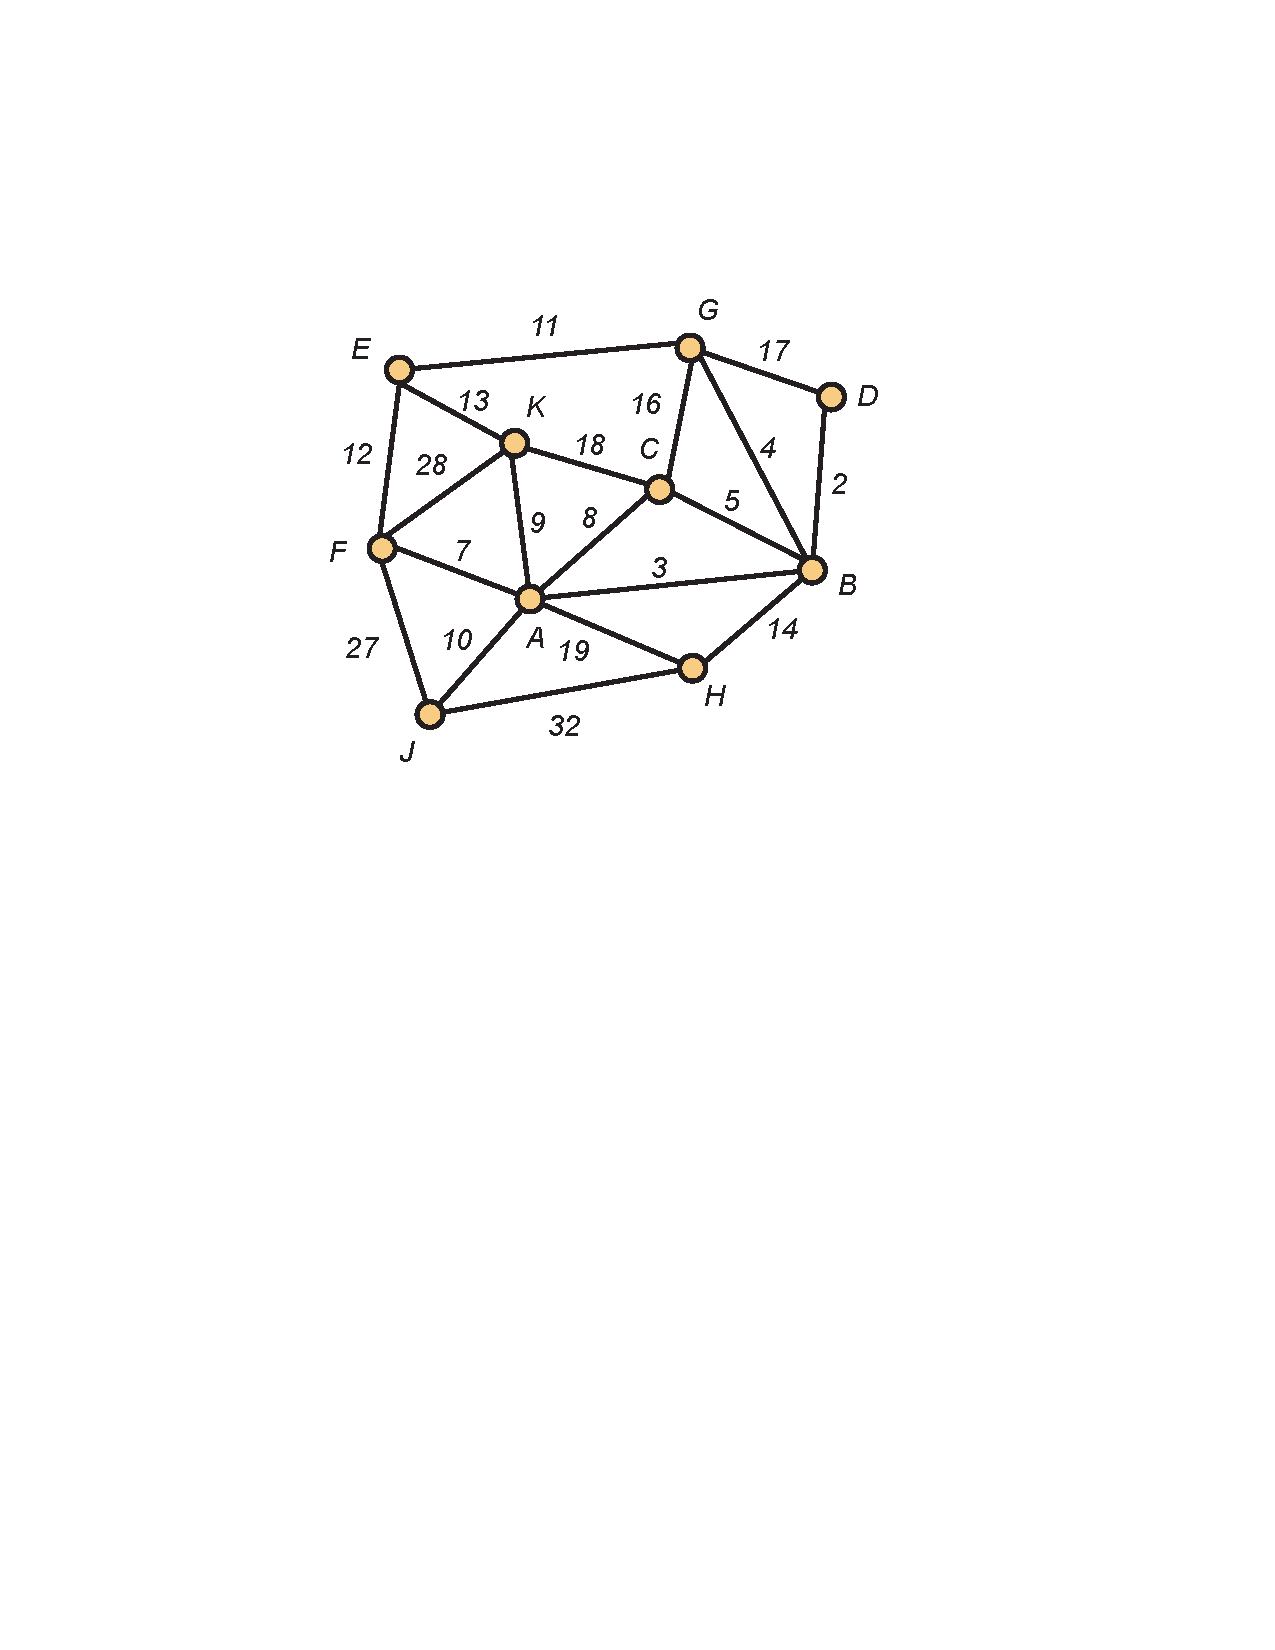
\includegraphics[viewport=140 413 430 650, scale=.6]{intro-figs/3012-fig12}\\
\end{center}
\caption{A labeled graph with weighted edges}
\label{fig:wgraph-1}
\end{figure}

Suppose the vertices are cities, the edges are highways
and the weights on the edges represent \textit{distance}.

\medskip
\noindent
$Q_1$:\quad  What is the shortest path from vertex~$E$ to vertex~$B$?

\medskip
Suppose Ariel is a salesperson whose home base is city~$A$. 

\medskip
\noindent
$Q_2$:\quad In what order should Ariel visit the other cities so that she
goes through each of them at least once and returns home
at the end---while keeping the total distance traveled to a minimum?  
Can Ariel accomplish such a tour visiting
each city \textit{exactly} once? 

\medskip
Sanjay is a highway inspection engineer and must traverse every
highway each month.  Sanjay's homebase is City~$E$.  

\medskip
\noindent
$Q_3$:\quad In what
order should Sanjay traverse the highways to minimize the total
distance traveled?  Can Sanjay make such a tour traveling
along each highway exactly once?
\end{example}

\begin{example}
  Now suppose that the vertices are locations of branch banks in
  Atlanta and that the weights on an edge represents the cost, in
  millions of dollars, of building a high capacity data link between
  the branch banks at it two end points.  In this model, if there is
  no edge between two branch banks, it means that the cost of building
  a data link between this particular pair is prohibitively high (here
  we might be tempted to say the cost is infinite, but the authors don't
  admit to knowing the meaning of this word).

  Our challenge is to decide which data links should be constructed to
  form a network in which any branch bank can communicate with any
  other branch.  We assume that data can flow in either direction on a
  link, should it be built, and that data can be relayed through any
  number of data links.  So to allow full communication, we should
  construct a \textit{spanning tree} in this network.  In
  \autoref{fig:spantree-1}, we show a graph $G$ on the left and one of
  its many \textit{spanning trees} on the right.

\begin{figure}
\begin{center}
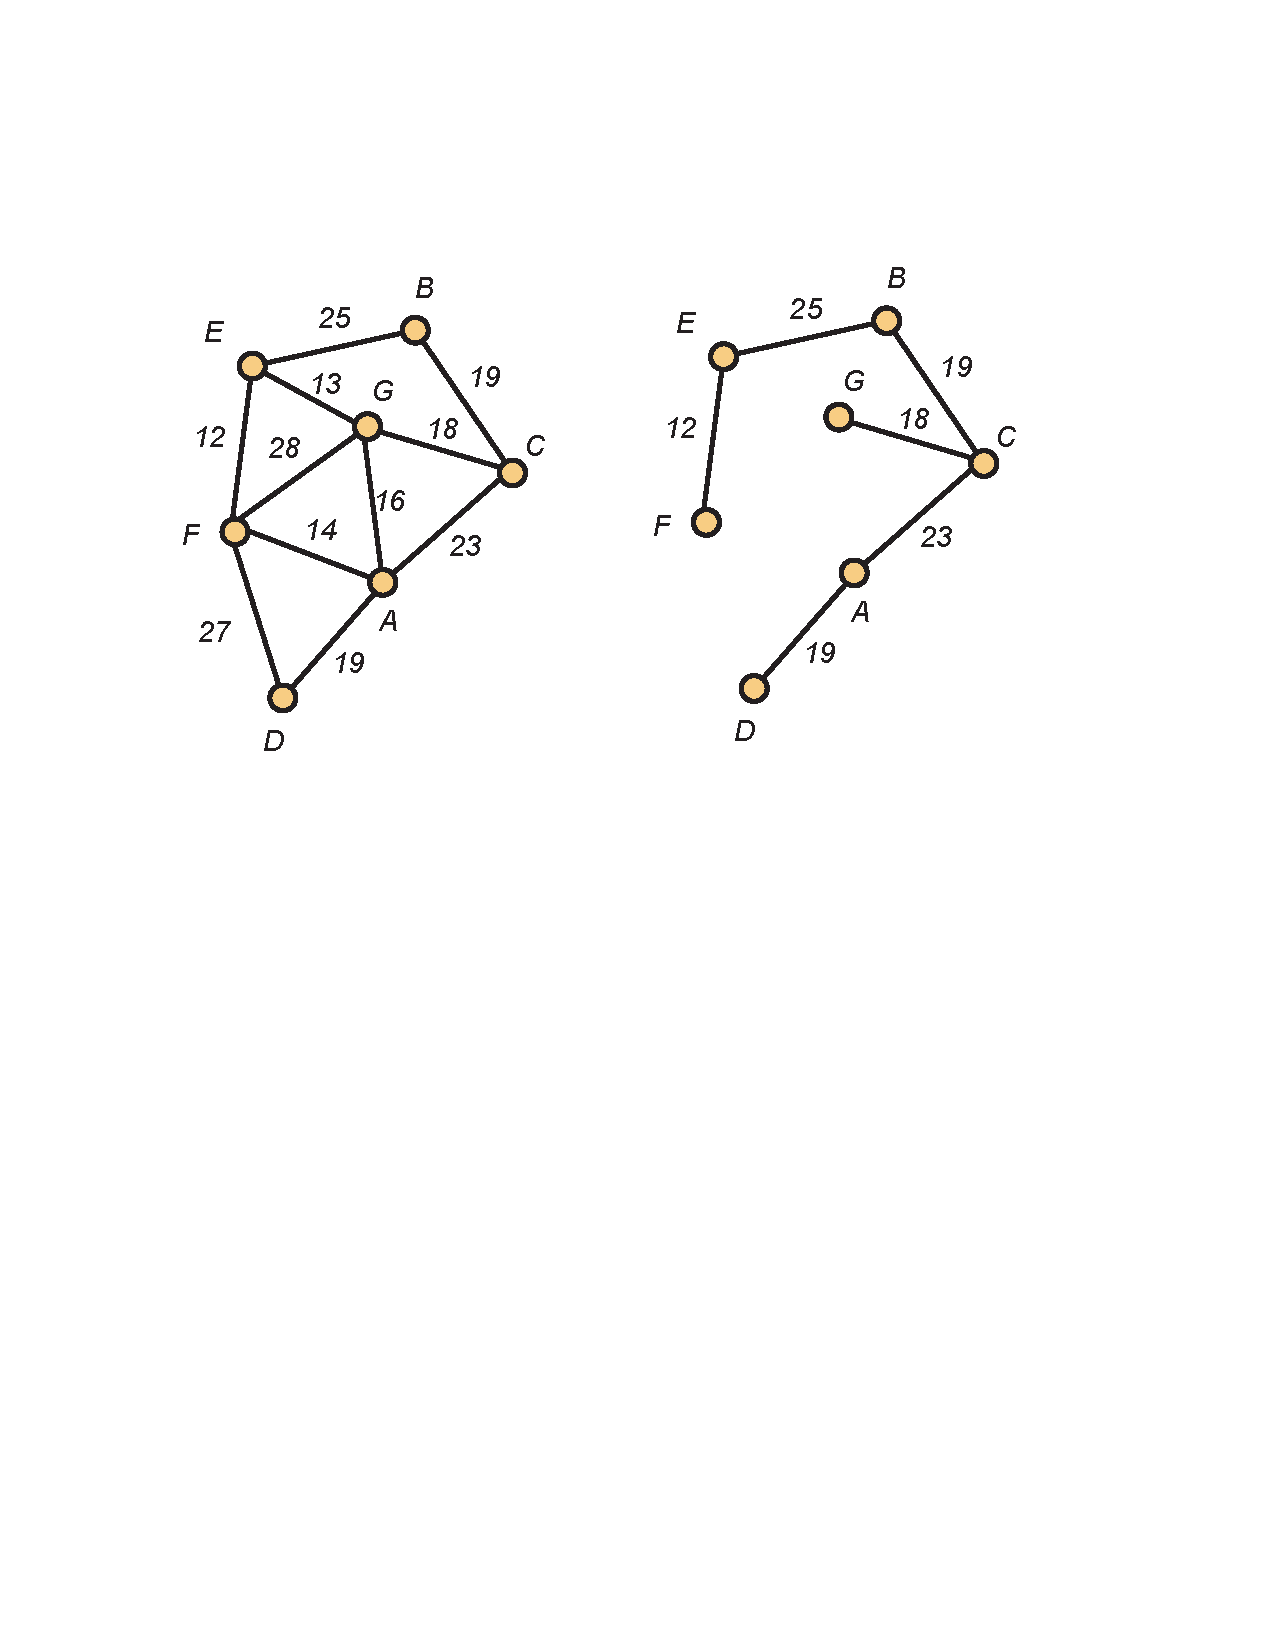
\includegraphics[viewport=82 420 500 677, scale=.6]{intro-figs/3012-fig19}\\
\end{center}
\caption{A weighted graph and spanning tree}
\label{fig:spantree-1}
\end{figure}

The weight of the spanning tree is the sum of the weights on the
edges.  In our model, this represents the costs, again in millions of
dollars, of building the data links associated with the edges in the
spanning tree.  For the spanning tree shown in
\autoref{fig:spantree-1}, this total is
\[
12+25+19+18+23+19 = 116.
\]
Of all spanning trees, the bank would naturally like to find one
having minimum weight.

How many spanning trees does this graph have?  For a large graph, say
one with $2875$ vertices, does it make sense to find all spanning
trees and simply take the one with minimum cost?  In particular, for a
positive integer~$n$, how many trees have vertex set
$\{1,2,3,\dots,n\}$?
\end{example}

\section{Sudoku Puzzles}\label{s:intro:sudoku}

Here's an example which has more substance than you might
think at first glance.  It involves Sudoku puzzles, which
have become immensely popular in recent years.
\begin{example}
  A Sudoku puzzle is a $9\times 9$ array of cells that when completed
  have the integers $1,2,\dots,9$ appearing exactly once in each row
  and each column.  Also (and this is what makes the puzzles so
  fascinating), the numbers $1$, $2$, $3,\dots,9$ appear once in each
  of the nine $3\times 3$ subquares identified by the darkened
  borders.  To be considered a legitimate Sudoku puzzle, there should
  be a \textit{unique} solution.  In \autoref{fig:sudoku}, we show two
  Sudoku puzzles.  The one on the right is fairly easy, and the one on
  the left is far more challenging.

\begin{figure}[hb]
\begin{center}
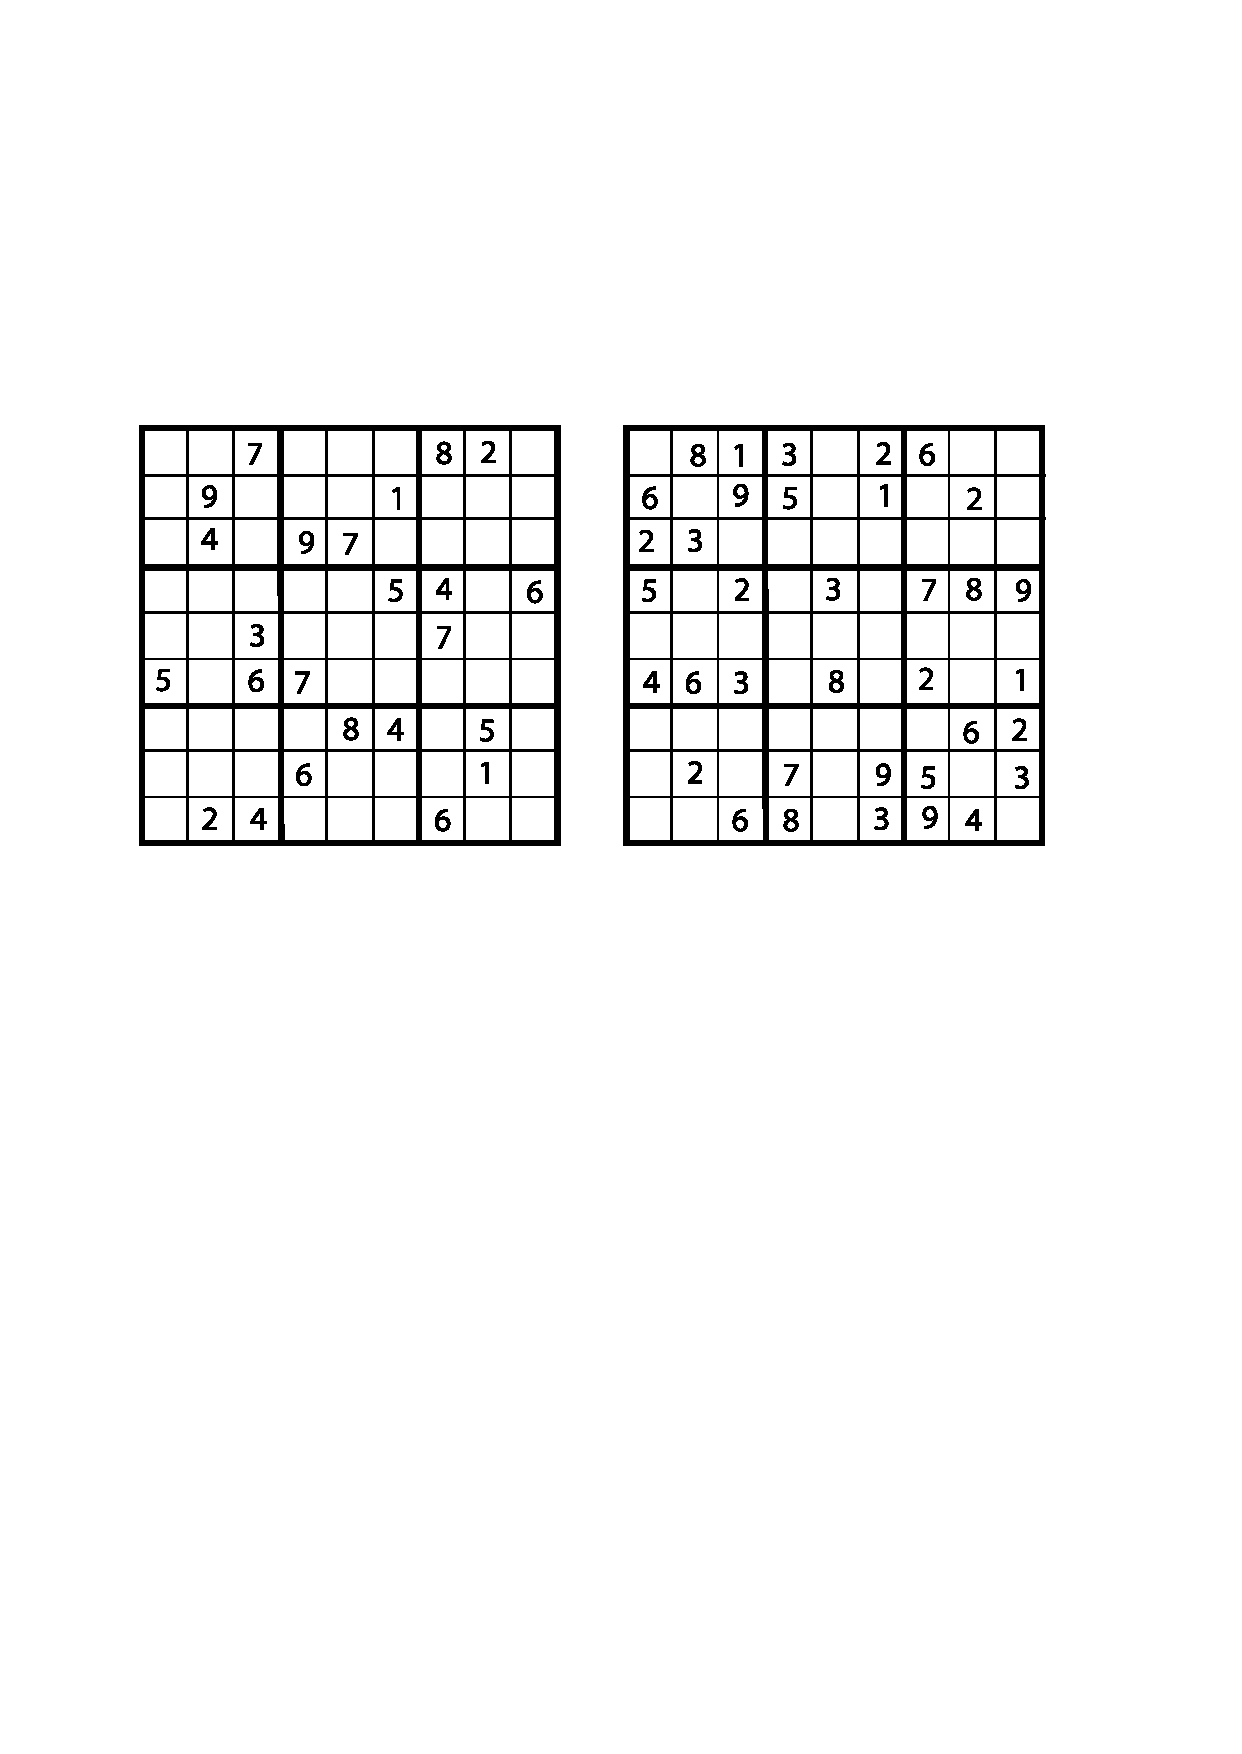
\includegraphics[viewport=60 428 509 645, scale=.8]{intro-figs/mysudoku}\\
\end{center}
\caption{Sudoku puzzles}
\label{fig:sudoku}
\end{figure}

There are many sources of Sudoku puzzles, and software that generates
Sudoku puzzles and then allows you to play them with an attractive GUI
is available for all operating systems we know anything about (although
not recommend to play them during class!).  Also, you can find 
Sudoku puzzles on the web at:

\medskip
\begin{center}
\href{http://www.websudoku.com}.
\end{center}

\medskip
\noindent
On this site, the ``Evil'' ones are just that.

How does Rory make up good Sudoku puzzles, ones that are difficult
for Mandy to solve?  How could Mandy use
a computer to solve puzzles that Rory has constructed? 
What makes some Sudoku puzzles easy and some of them hard?

The size of a Sudoku puzzle can be expanded in an obvious
way, and many newspapers include a $16\times16$ Sudoku puzzle
in their Sunday edition (just next to a challenging crosswords puzzle).
How difficult would it be to solve a $1024\times1024$ Sudoku puzzle,
even if you had access to a powerful computer?
\end{example}

\section{Discussion}\label{s:intro:closing}

Over coffee after their first combinatorics class, Xing remarked
''This doesn't seem to be going like calculus.  I'm expecting
the professor to teach us how to solve problems---at least some
kinds of problems.  Instead, a whole bunch
of problems were posed and we were asked whether 
\textit{we} could solve them.'' Yolanda jumped in ``You may be 
judging things too quickly.  I'm fascinated by these kinds
of questions.  They're different.''  Zori grumpily layed
bare her concerns
``After getting out of Georgia Tech, who's going to pay me to
count necklaces, distribute library books or solve Sudoku puzzles.''
Bob politely countered ``But the problems on networks and graphs
seemed to have practical applications.  I heard my uncle, a very
successful business guy, talk about franchising problems that
sound just like those.''  Alice speculated ``All those network problems
sound the same to me.  A fair to middling computer science major could 
probably write programs to solve any of them.''  Dave mumbled ``Maybe not.
Similar sounding problems might actually be quite different in the end.  
Maybe we'll learn to tell the difference.'' 
After a bit of quiet time interrupted only by latte's disappearing,
Carlos said softly ``It might not be so easy to distinguish hard 
problems from easy ones.'' Alice followed ``Regardless, what strikes 
me is that we all,  well almost all of us,''
she said, rolling her eyes at Bob ``seem to understand everything talked 
about in class today.  It was so very concrete. I liked that.''

%%% Local Variables: 
%%% mode: latex
%%% TeX-master: "book"
%%% End: 
